
\chapter{2. Linear PDEs, naively}

We start with a cliched example because it is the right place to start.

\section{A finite element method for the Poisson problem}

Let $\Omega \subset \RR^d$ be a region\marginnote{Only $d=2$ and $d=3$ are used in this book.} with boundary decomposed into well-behaved subsets $\partial_D \Omega$ and $\partial_N \Omega$ whose union is the whole boundary $\partial \Omega$.  The \emph{Poisson problem}, in strong form and including both Dirichlet and Neumann boundary conditions, is
\begin{align}
- \grad^2 u &= f \quad \text{ on } \Omega, \label{poissonstrong} \\
u &= g \quad \text{ on } \partial_D \Omega, \notag \\
\frac{\partial u}{\partial n} &= h \quad \text{ on } \partial_N \Omega \notag
\end{align}
where $\partial u/\partial n = \bn \cdot \grad u$ and $\bn$ is the outward unit normal on $\partial \Omega$.\marginnote{%
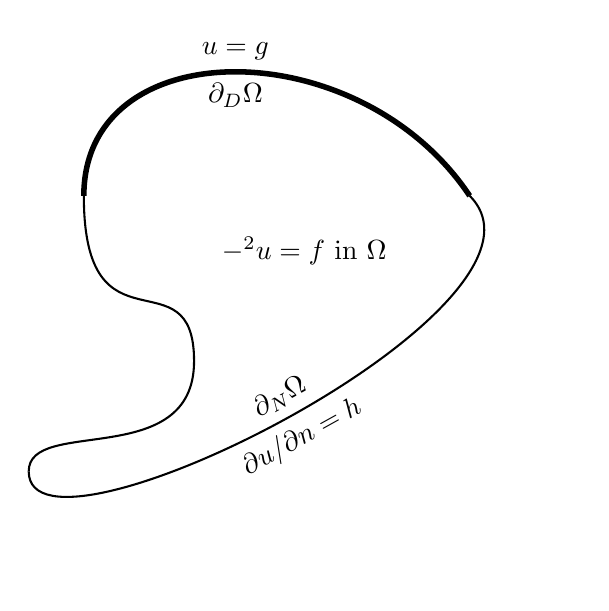
\begin{tikzpicture}[scale=0.7]
%\draw[gray,very thin] (-2,-7) grid (9,4);
\draw[line width=2pt] (0,0) .. controls (0,3) and (5,3) .. node[sloped,above] {$u=g$} node[sloped,below] {$\partial_D\Omega$} (7,0);
\draw[line width=0.75pt] (7,0) .. controls (9,-2) and (-1,-7) .. node[sloped,above] {$\partial_N\Omega$} node[sloped,below] {$\partial u/\partial n = h$} (-1,-5);
\draw[line width=0.75pt] (-1,-5) .. controls (-1,-4) and (2,-5) .. (2,-3);
\draw[line width=0.75pt] (2,-3) .. controls (2,-1) and (0,-3) .. (0,0);
\draw[line width=0.75pt] (4,-1) node {$- \grad^2 u = f$ in $\Omega$};
\end{tikzpicture}}

The data of problem \eqref{poissonstrong}, besides the region $\Omega$ and its boundary, is a \emph{source term} $f\in L^2(\Omega)$, \emph{Dirichlet data} $g\in L^2(\partial_N \Omega)$, and \emph{non-homogeneous Neumann data} $h\in L^2(\partial_N \Omega)$.  For simplicity, and so that the solution of this problem is unique if it exists \citep{Elmanetal2005}, we assume $\partial_D \Omega$ has positive measure.  All of our examples will have that property.

The Poisson problem models the distribution of temperature in a conducting object at steady state, the electrostatic potential, the equilibrium distribution from certain random walks, and many other other physical phenomena.  And it is linear, that is, if $u_1$ and $u_2$ are solutions then convex linear combinations are also solutions.  More relevantly, it is a linear problem in the sense that finite-dimensional approximations of the Poisson problem are simply matrix problems.

As \eqref{poissonstrong} is stated there may be no solution where ``$\grad^2 u$'' makes sense as a function.  In particular, there may be no $u\in C^2(\Omega)$ which is continuous up to the boundary (i.e.~$u\in C(\bar\Omega)$).  There is, however, a unique solution\sidenote{Many mathematical concepts, including a well-posedness proof that justifies this claim, are all covered by \citep{Evans}.  These are technicalities for us.  Our goal is computational performance in cases where the Poisson problem is mathematically well-behaved.} if we change to a \emph{weak formulation}.  We will state the weak formulation after defining function spaces.

Let
    $$H^1(\Omega) = \{u\in L^2(\Omega) \big| \grad u \text{ exists a.e.~and } \grad u \in L^2(\Omega)\},$$
a Sobolev space \citep{Evans}.  This space has two subsets we will use, namely functions with value $g$ and those with value $0$ on $\partial_D \Omega$, respectively, which we denote $H_g^1(\Omega)$ and $H_0^1(\Omega)$.

The weak formulation of \eqref{poissonstrong} comes from choosing any $v\in H_0^1(\Omega)$, multiplying the first equation in \eqref{poissonstrong} by $v$, and integrating by parts:
\begin{equation*}
\int_\Omega \grad u \cdot \grad v - \int_{\partial\Omega} \frac{\partial u}{\partial n} v = \int_\Omega f v.
\end{equation*}
Now,\marginnote{%
{\color{red}The main ideas} of strong and weak formulations:\begin{itemize}
\item If $u \in H_g^1(\Omega)$ solves the strong form \eqref{poissonstrong} then it solves \eqref{poissonweak} also.
\item If $u \in H_g^1(\Omega)$ solves the weak form \eqref{poissonweak} then we accept it, by definition, as a solution of the Poisson problem.\end{itemize}}
supposing we already have a classical solution $u$ of \eqref{poissonstrong}, which is in $H_g^1(\Omega)$, we use the fact that $v=0$ on $\partial_D\Omega$ and the Neumann data:
\begin{equation}
\int_\Omega \grad u \cdot \grad v = \int_\Omega f v + \int_{\partial_N\Omega} h v\quad \text{ for any } v\in H_0^1(\Omega). \label{poissonweak}
\end{equation}

Equation \eqref{poissonweak} is the weak formulation of the Poisson problem.  A key observation is that $u$ itself satisfies the Dirichlet boundary condition because it lives in $H_g^1(\Omega)$, while Neumann boundary data $h$, like the source function $f$, appears directly in \eqref{poissonweak}.

The \emph{finite element method} (FEM) comes from requiring the weak formulation for $u$ in a finite-dimensional subset of $H_g^1(\Omega)$, and for $v$ in a finite-dimensional subspace of $H_0^1(\Omega)$; more precisely, this is a \emph{Galerkin} FEM.  We will build these finite-dimensional subsets, in the current example, using a \emph{unstructured triangulation} on a region $\Omega\subset \RR^2$

To make this work, from now on we require that $\Omega$ be polygonal,\marginnote{%
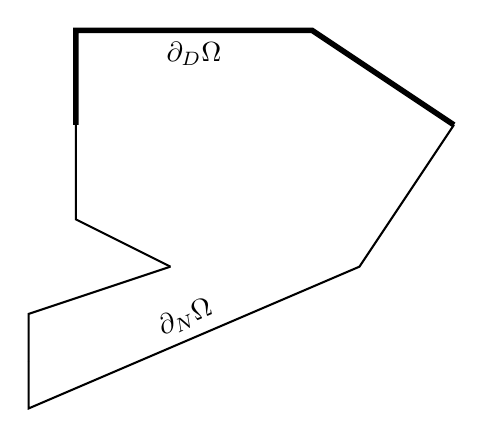
\begin{tikzpicture}[scale=0.6]
%\draw[gray,very thin] (-2,-7) grid (9,4);
\draw[line width=2pt] (0,0) -- (0,2) -- node[sloped,below] {$\partial_D\Omega$} (5,2) -- (8,0);
\draw[line width=0.75pt] (8,0) -- (6,-3) -- node[sloped,above] {$\partial_N\Omega$} (-1,-6) -- (-1,-5);
\draw[line width=0.75pt] (-1,-5) -- (-1,-4) -- (2,-3);
\draw[line width=0.75pt] (2,-3) -- (0,-2) -- (0,0);
\end{tikzpicture}}
 with boundary $\partial\Omega$ a closed polygon whose sides are each of positive length, and whose sides are either entirely in $\partial_D\Omega$ or in $\partial_N\Omega$.  As before, to produce a unique solution we require that $\partial_D\Omega$ contain at least one such side.

The triangulation itself is a set

once we have a triangulation
\begin{marginfigure}
% created by script tri2tikz.py command line:
%   ./tri2tikz.py --labelnodes --scale 2.0 --labeloffset 0.25 bump.1 bump.1.tikz
%
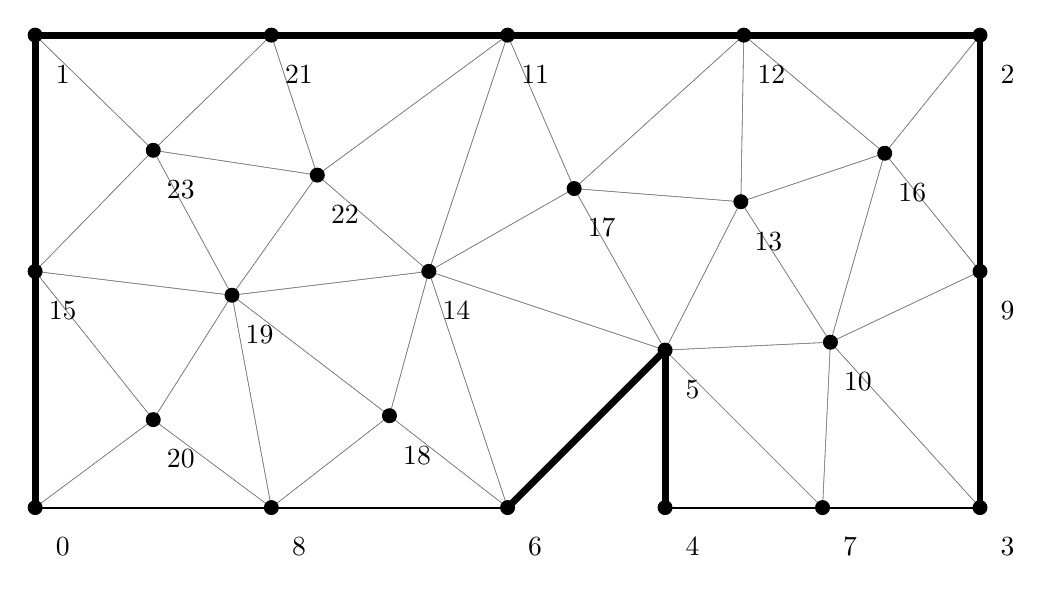
\begin{tikzpicture}[scale=2.000000]
  \draw[gray,very thin] (-1.500000,0.000000) -- (-2.250000,0.558372);
  \draw[gray,very thin] (-2.250000,0.558372) -- (-3.000000,0.000000);
  \draw[gray,very thin] (-3.000000,0.000000) -- (-1.500000,0.000000);
  \draw[gray,very thin] (-1.500000,0.000000) -- (0.000000,0.000000);
  \draw[gray,very thin] (0.000000,0.000000) -- (-0.750000,0.583333);
  \draw[gray,very thin] (-0.750000,0.583333) -- (-1.500000,0.000000);
  \draw[gray,very thin] (1.481325,1.942169) -- (0.422665,2.025778);
  \draw[gray,very thin] (0.422665,2.025778) -- (1.000000,1.000000);
  \draw[gray,very thin] (1.000000,1.000000) -- (1.481325,1.942169);
  \draw[gray,very thin] (-0.500000,1.500000) -- (0.000000,0.000000);
  \draw[gray,very thin] (0.000000,0.000000) -- (1.000000,1.000000);
  \draw[gray,very thin] (1.000000,1.000000) -- (-0.500000,1.500000);
  \draw[gray,very thin] (0.000000,3.000000) -- (-1.500000,3.000000);
  \draw[gray,very thin] (-1.500000,3.000000) -- (-1.208263,2.111158);
  \draw[gray,very thin] (-1.208263,2.111158) -- (0.000000,3.000000);
  \draw[gray,very thin] (2.000000,0.000000) -- (2.050000,1.050000);
  \draw[gray,very thin] (2.050000,1.050000) -- (1.000000,1.000000);
  \draw[gray,very thin] (1.000000,1.000000) -- (2.000000,0.000000);
  \draw[gray,very thin] (1.000000,0.000000) -- (2.000000,0.000000);
  \draw[gray,very thin] (2.000000,0.000000) -- (1.000000,1.000000);
  \draw[gray,very thin] (1.000000,1.000000) -- (1.000000,0.000000);
  \draw[gray,very thin] (2.394659,2.250000) -- (3.000000,1.500000);
  \draw[gray,very thin] (3.000000,1.500000) -- (3.000000,3.000000);
  \draw[gray,very thin] (3.000000,3.000000) -- (2.394659,2.250000);
  \draw[gray,very thin] (1.500000,3.000000) -- (0.422665,2.025778);
  \draw[gray,very thin] (0.422665,2.025778) -- (1.481325,1.942169);
  \draw[gray,very thin] (1.481325,1.942169) -- (1.500000,3.000000);
  \draw[gray,very thin] (2.050000,1.050000) -- (3.000000,0.000000);
  \draw[gray,very thin] (3.000000,0.000000) -- (3.000000,1.500000);
  \draw[gray,very thin] (3.000000,1.500000) -- (2.050000,1.050000);
  \draw[gray,very thin] (2.394659,2.250000) -- (2.050000,1.050000);
  \draw[gray,very thin] (2.050000,1.050000) -- (3.000000,1.500000);
  \draw[gray,very thin] (3.000000,1.500000) -- (2.394659,2.250000);
  \draw[gray,very thin] (-1.500000,3.000000) -- (-3.000000,3.000000);
  \draw[gray,very thin] (-3.000000,3.000000) -- (-2.250000,2.268853);
  \draw[gray,very thin] (-2.250000,2.268853) -- (-1.500000,3.000000);
  \draw[gray,very thin] (1.481325,1.942169) -- (1.000000,1.000000);
  \draw[gray,very thin] (1.000000,1.000000) -- (2.050000,1.050000);
  \draw[gray,very thin] (2.050000,1.050000) -- (1.481325,1.942169);
  \draw[gray,very thin] (3.000000,0.000000) -- (2.050000,1.050000);
  \draw[gray,very thin] (2.050000,1.050000) -- (2.000000,0.000000);
  \draw[gray,very thin] (2.000000,0.000000) -- (3.000000,0.000000);
  \draw[gray,very thin] (0.422665,2.025778) -- (1.500000,3.000000);
  \draw[gray,very thin] (1.500000,3.000000) -- (0.000000,3.000000);
  \draw[gray,very thin] (0.000000,3.000000) -- (0.422665,2.025778);
  \draw[gray,very thin] (2.394659,2.250000) -- (1.500000,3.000000);
  \draw[gray,very thin] (1.500000,3.000000) -- (1.481325,1.942169);
  \draw[gray,very thin] (1.481325,1.942169) -- (2.394659,2.250000);
  \draw[gray,very thin] (-1.750000,1.348485) -- (-0.750000,0.583333);
  \draw[gray,very thin] (-0.750000,0.583333) -- (-0.500000,1.500000);
  \draw[gray,very thin] (-0.500000,1.500000) -- (-1.750000,1.348485);
  \draw[gray,very thin] (-1.500000,0.000000) -- (-0.750000,0.583333);
  \draw[gray,very thin] (-0.750000,0.583333) -- (-1.750000,1.348485);
  \draw[gray,very thin] (-1.750000,1.348485) -- (-1.500000,0.000000);
  \draw[gray,very thin] (1.500000,3.000000) -- (2.394659,2.250000);
  \draw[gray,very thin] (2.394659,2.250000) -- (3.000000,3.000000);
  \draw[gray,very thin] (3.000000,3.000000) -- (1.500000,3.000000);
  \draw[gray,very thin] (2.050000,1.050000) -- (2.394659,2.250000);
  \draw[gray,very thin] (2.394659,2.250000) -- (1.481325,1.942169);
  \draw[gray,very thin] (1.481325,1.942169) -- (2.050000,1.050000);
  \draw[gray,very thin] (0.000000,3.000000) -- (-0.500000,1.500000);
  \draw[gray,very thin] (-0.500000,1.500000) -- (0.422665,2.025778);
  \draw[gray,very thin] (0.422665,2.025778) -- (0.000000,3.000000);
  \draw[gray,very thin] (1.000000,1.000000) -- (0.422665,2.025778);
  \draw[gray,very thin] (0.422665,2.025778) -- (-0.500000,1.500000);
  \draw[gray,very thin] (-0.500000,1.500000) -- (1.000000,1.000000);
  \draw[gray,very thin] (0.000000,0.000000) -- (-0.500000,1.500000);
  \draw[gray,very thin] (-0.500000,1.500000) -- (-0.750000,0.583333);
  \draw[gray,very thin] (-0.750000,0.583333) -- (0.000000,0.000000);
  \draw[gray,very thin] (-1.750000,1.348485) -- (-2.250000,2.268853);
  \draw[gray,very thin] (-2.250000,2.268853) -- (-3.000000,1.500000);
  \draw[gray,very thin] (-3.000000,1.500000) -- (-1.750000,1.348485);
  \draw[gray,very thin] (-3.000000,1.500000) -- (-3.000000,0.000000);
  \draw[gray,very thin] (-3.000000,0.000000) -- (-2.250000,0.558372);
  \draw[gray,very thin] (-2.250000,0.558372) -- (-3.000000,1.500000);
  \draw[gray,very thin] (-1.500000,0.000000) -- (-1.750000,1.348485);
  \draw[gray,very thin] (-1.750000,1.348485) -- (-2.250000,0.558372);
  \draw[gray,very thin] (-2.250000,0.558372) -- (-1.500000,0.000000);
  \draw[gray,very thin] (-3.000000,1.500000) -- (-2.250000,0.558372);
  \draw[gray,very thin] (-2.250000,0.558372) -- (-1.750000,1.348485);
  \draw[gray,very thin] (-1.750000,1.348485) -- (-3.000000,1.500000);
  \draw[gray,very thin] (0.000000,3.000000) -- (-1.208263,2.111158);
  \draw[gray,very thin] (-1.208263,2.111158) -- (-0.500000,1.500000);
  \draw[gray,very thin] (-0.500000,1.500000) -- (0.000000,3.000000);
  \draw[gray,very thin] (-0.500000,1.500000) -- (-1.208263,2.111158);
  \draw[gray,very thin] (-1.208263,2.111158) -- (-1.750000,1.348485);
  \draw[gray,very thin] (-1.750000,1.348485) -- (-0.500000,1.500000);
  \draw[gray,very thin] (-2.250000,2.268853) -- (-1.208263,2.111158);
  \draw[gray,very thin] (-1.208263,2.111158) -- (-1.500000,3.000000);
  \draw[gray,very thin] (-1.500000,3.000000) -- (-2.250000,2.268853);
  \draw[gray,very thin] (-3.000000,1.500000) -- (-2.250000,2.268853);
  \draw[gray,very thin] (-2.250000,2.268853) -- (-3.000000,3.000000);
  \draw[gray,very thin] (-3.000000,3.000000) -- (-3.000000,1.500000);
  \draw[gray,very thin] (-1.208263,2.111158) -- (-2.250000,2.268853);
  \draw[gray,very thin] (-2.250000,2.268853) -- (-1.750000,1.348485);
  \draw[gray,very thin] (-1.750000,1.348485) -- (-1.208263,2.111158);
  \draw[line width=2.5pt] (-3.000000,0.000000) -- (-3.000000,1.500000);
  \draw[line width=2.5pt] (-3.000000,3.000000) -- (-1.500000,3.000000);
  \draw[line width=2.5pt] (3.000000,3.000000) -- (3.000000,1.500000);
  \draw[line width=0.75pt] (3.000000,0.000000) -- (2.000000,0.000000);
  \draw[line width=0.75pt] (2.000000,0.000000) -- (1.000000,0.000000);
  \draw[line width=2.5pt] (1.000000,1.000000) -- (1.000000,0.000000);
  \draw[line width=2.5pt] (0.000000,0.000000) -- (1.000000,1.000000);
  \draw[line width=0.75pt] (0.000000,0.000000) -- (-1.500000,0.000000);
  \draw[line width=0.75pt] (-1.500000,0.000000) -- (-3.000000,0.000000);
  \draw[line width=2.5pt] (3.000000,1.500000) -- (3.000000,0.000000);
  \draw[line width=2.5pt] (0.000000,3.000000) -- (1.500000,3.000000);
  \draw[line width=2.5pt] (1.500000,3.000000) -- (3.000000,3.000000);
  \draw[line width=2.5pt] (-3.000000,1.500000) -- (-3.000000,3.000000);
  \draw[line width=2.5pt] (-1.500000,3.000000) -- (0.000000,3.000000);
  \draw (-2.825000,-0.250000) node {$0$};
  \filldraw (-3.000000,0.000000) circle (1.25pt);
  \draw (-2.825000,2.750000) node {$1$};
  \filldraw (-3.000000,3.000000) circle (1.25pt);
  \draw (3.175000,2.750000) node {$2$};
  \filldraw (3.000000,3.000000) circle (1.25pt);
  \draw (3.175000,-0.250000) node {$3$};
  \filldraw (3.000000,0.000000) circle (1.25pt);
  \draw (1.175000,-0.250000) node {$4$};
  \filldraw (1.000000,0.000000) circle (1.25pt);
  \draw (1.175000,0.750000) node {$5$};
  \filldraw (1.000000,1.000000) circle (1.25pt);
  \draw (0.175000,-0.250000) node {$6$};
  \filldraw (0.000000,0.000000) circle (1.25pt);
  \draw (2.175000,-0.250000) node {$7$};
  \filldraw (2.000000,0.000000) circle (1.25pt);
  \draw (-1.325000,-0.250000) node {$8$};
  \filldraw (-1.500000,0.000000) circle (1.25pt);
  \draw (3.175000,1.250000) node {$9$};
  \filldraw (3.000000,1.500000) circle (1.25pt);
  \draw (2.225000,0.800000) node {$10$};
  \filldraw (2.050000,1.050000) circle (1.25pt);
  \draw (0.175000,2.750000) node {$11$};
  \filldraw (0.000000,3.000000) circle (1.25pt);
  \draw (1.675000,2.750000) node {$12$};
  \filldraw (1.500000,3.000000) circle (1.25pt);
  \draw (1.656325,1.692169) node {$13$};
  \filldraw (1.481325,1.942169) circle (1.25pt);
  \draw (-0.325000,1.250000) node {$14$};
  \filldraw (-0.500000,1.500000) circle (1.25pt);
  \draw (-2.825000,1.250000) node {$15$};
  \filldraw (-3.000000,1.500000) circle (1.25pt);
  \draw (2.569659,2.000000) node {$16$};
  \filldraw (2.394659,2.250000) circle (1.25pt);
  \draw (0.597665,1.775778) node {$17$};
  \filldraw (0.422665,2.025778) circle (1.25pt);
  \draw (-0.575000,0.333333) node {$18$};
  \filldraw (-0.750000,0.583333) circle (1.25pt);
  \draw (-1.575000,1.098485) node {$19$};
  \filldraw (-1.750000,1.348485) circle (1.25pt);
  \draw (-2.075000,0.308372) node {$20$};
  \filldraw (-2.250000,0.558372) circle (1.25pt);
  \draw (-1.325000,2.750000) node {$21$};
  \filldraw (-1.500000,3.000000) circle (1.25pt);
  \draw (-1.033263,1.861158) node {$22$};
  \filldraw (-1.208263,2.111158) circle (1.25pt);
  \draw (-2.075000,2.018853) node {$23$};
  \filldraw (-2.250000,2.268853) circle (1.25pt);
\end{tikzpicture}

\caption{A FEM triangulation}
\label{fig:triangulation}
\end{marginfigure}

\marginnote{{\color{red} Remember:} $u_h$ is the \emph{trial} function and $v_h$ are the \emph{test} functions}

%\vspace{4.0in}

\section{Getting a triangular mesh into \PETSc}

\cinputpart{c2triangle.c}{The standard preamble.}{I}{//STARTPREAMBLE}{//ENDPREAMBLE}

\cinputpart{c2triangle.c}{Determine filenames using \PETSc option processing.}{II}{//ENDPREAMBLE}{//ENDFILENAME}

\cinputpart{c2triangle.c}{Start to read ASCII files with \textsc{triangle}-generated mesh by going to rank zero processor, reading node header, and allocating accordingly.}{III}{//ENDFILENAME}{//ENDRANK0ALLOC}

\cinputpart{c2triangle.c}{On rank zero processor: Read node information.}{IV}{//ENDRANK0ALLOC}{//ENDREADNODES}

\cinputpart{c2triangle.c}{On rank zero processor: Read element information.}{V}{//ENDREADNODES}{//ENDREADELEMENTS}

\cinputpart{c2triangle.c}{On rank zero processor: Write the mesh out in \PETSc binary format.}{VI}{//ENDREADELEMENTS}{//ENDRANK0}

\cinputpart{c2triangle.c}{Re-read mesh in parallel, and write in parallel.}{VII}{//ENDRANK0}{//END}


\section{FEM method, for the Poisson equation}

\section{Preallocate a \pMat}

%\cinputfull{c2prealloc.c}{demonstrates preallocation of parallel \pMat}{}{}

\section{Assembling Poisson}

\section{Performance: convergence and scaling}

\caveat{But real-world PDEs are nonlinear.}
